We will now introduce the general theory of linear response, also referred to as the Kubo formalism.
Later, the theory will be specialized to thermoelectric response.
The material of this section is mostly inspired by the explanations given in~\citeauthor{giulianiQuantumTheoryElectron2005}~\cite{giulianiQuantumTheoryElectron2005}.
The specialization to the electric response and Luttinger's method is also inspired by~\citeauthor{mahanManyparticlePhysics2000}~\cite{mahanManyparticlePhysics2000}.

\todo{Consider making this discussion in both time and space}

We are interested in expressing the response of the observable ${A}$ to some field $F$ coupling to another observable ${B}$.
Let the uncoupled system be described by the Hamiltonian $H_{0}$ and the coupling term be $H_F = F(t) {B}$.
Assume also that the coupling field $F$ is turned on at $t=t_0$,  such that $H_F(t) = 0$ for $t < t_0$.
Let the unperturbed Hamiltonian be $H_0$, which will be assumed time independent.
The total Hamiltonian describing the coupled system is
\begin{equation}
  \label{eq:kubo-perturbation}
{H}(t) = H_0 + H_F = H_0+ F(t) {B}.
\end{equation}
Linear response theory tells us then that the response $\delta {A}$ is given by~\cite{giulianiQuantumTheoryElectron2005}
\begin{equation}\label{eq:lin-response-1}
  \delta {A} = -\frac{i}{\hbar} \int\limits_{t_0}^t
  \Braket{\left[
{A}(t), {B}(t')
\right]}_{0}
F(t') \mathrm{dt'},
\end{equation}
where $[{A}, {B}]$ is the operator commutator and $\braket{\dots}_0$ denotes the average in the thermal equilibrium ensemble.
A  non-rigorous motivation for this form of the response is the fact that
\begin{equation}
  \dot{{A}} = -\frac{i}{\hbar } \left[ {A}, H \right]
  + \frac{\partial {A}_{S}}{\partial t}, 
\end{equation}
with $A_S$ the Schrödinger picture operator, whose derivative is from here on assumed zero.
Taking $H=H_F$, the part of the Hamiltonian whose dynamics we are interested in, and integrate over the interaction time, the result is reminiscent of Eq.~(\ref{eq:lin-response-1}).
For a proper derivation see for example~\citeauthor{giulianiQuantumTheoryElectron2005}~\cite[Chapter 3.3]{giulianiQuantumTheoryElectron2005}.
\todo{Note about time dependent vs independent operators/picture ? see Giuliani and Vaginal (3.29).}
\todo{Some other formulation for what the $\braket\dots_0$ means.}

We will now try to make this expression slightly more manageable, and in the process we will highlight some important physical properties of the expression.
Firstly, by taking advantage of the time translation invariance of the uncoupled Hamiltonian $H_0$, we may realize that the average taken in the unperturbed basis may be taken at a more convenient time, preserving the time separation of the operators
\begin{equation}
  \Braket{\left[
      {A}(t), {B}(t')
    \right]}_0
=
\Braket{\left[
    {A}(t-t'), {B}(0)
    \right]}_0.
\end{equation}
Inserting this back to Eq. (\ref{eq:lin-response-1}), and performing a change of variable $\tau = t  - t'$ we have
\begin{equation}
\label{eq:13}
\delta {A} = -\frac{i}{\hbar} \int\limits_{0}^{t-t_0}
\Braket{\left[
    {A}(\tau), {B}(0)
  \right]}_{0}
F(t - \tau) \mathrm{d\tau}.
\end{equation}
In this form the retardedness of the coupling is apparent -- no observable can be affected by a future perturbation, shown schematically in Figure \ref{fig:interaction}.

\begin{figure}[ht]
  \centering
    \resizebox{\textwidth}{!}{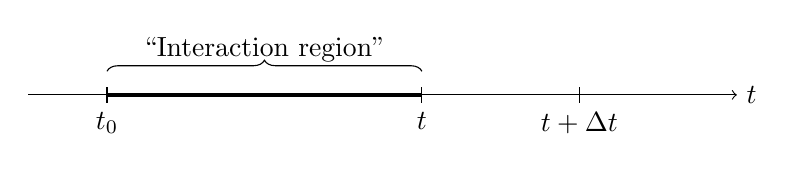
\begin{tikzpicture}
        \draw[->] (-5, 0) -- (4, 0) node[right]{$t$};
        \draw (-4, 0) +(0, 0.1) -- +(0, -0.1) node[below] {$t_0$};
        \draw (0, 0) +(0, 0.1) -- +(0, -0.1) node[below] {$t$};
        \draw (2, 0) +(0, 0.1) -- +(0, -0.1) node[below] {$t+\Delta t$};

        \draw[very thick] (-4, 0) -- (0,0);
        \draw[decorate, decoration={brace, amplitude=4pt}] (-4, 0.3) -- (0, 0.3) node[midway, above] {``Interaction region''};
      \end{tikzpicture}
    }
  \caption{Interacting region of a perturbation turned on at $t_0$. Note that the perturbation in the future, $t+\Delta t$, does not interact, as this is the retarded interaction.}
  \label{fig:interaction}
\end{figure}
For future convenience, and convention, we will in this last step introduce the \emph{response function}
\begin{equation}
\label{eq:14}
\chi_{AB}(\tau) = -\frac{i}{\hbar} \Theta(\tau)
\Braket{\left[
{A}(\tau), {B}(0)
  \right]}_0,
\end{equation}
where the step-function $\Theta$ was introduced to make the response function explicitly \emph{retarded}.
Then our final expression for the response of ${A}$ is
\begin{equation}
  \label{eq:linearResponse}
\delta {A} = \int\limits_{0}^{t-t_0}
\chi_{AB}(\tau) F(t - \tau) \mathrm{d\tau}.
\end{equation}
Note of course that the limits could be altered to $\int_{-\infty}^{\infty}$ given that the coupling field is zero for times earlier than $t_0$ and we have chosen the retarded response function.

\section[Charge response from electromagnetic coupling]{Linear response in charge current from electromagnetic coupling}
We will now discuss the electric \emph{conductivity} in light of the Kubo formalism, as an example to better understand and demonstrate the preceding discussion.
Firstly the concept of conductivity will be presented, then it will be derived using the machinery of the Kubo formula.
As mentioned above, this part follow the derivation of~\citeauthor{mahanManyparticlePhysics2000}~\cite{mahanManyparticlePhysics2000}.

The charge current $\vec{J}$ that is induced from an electric field $\vec{E}$ in the linear scheme is expressed by Ohm's law
\begin{equation}
  \label{eq:ohm}
  \vec{J}_i(\vec{r}, t) =
  \int\limits_{V} \mathrm{d} \vec{x} \!\int\limits_{-\infty}^t \mathrm{dt} \;
  \sigma_{ij}(\vec{r}, t, \vec{x}, s)
  \vec{E}_j(\vec{x}, s).
\end{equation}
Above the Einstein summation convention is used, and $\sigma$ is the \emph{conductivity tensor}.
We see of course that this has the familiar form of a response relation.
In the case of a simple and isotropic material, meaning symmetric under SO(n) and with no transverse response, the tensor is diagonal with $\vec{\sigma} = \sigma I$ and one gets the more well-known version of Ohm's law $\vec{J} = \sigma \vec{E}$.

Again, by the principle of causality, the response of $\vec{J}$ can only depend on $\vec{E}$ in the \emph{past};
thus $\sigma_{ij}(\vec{r}, t, \vec{x}, s)$ can be finite only where the time separation $t-s$ is less than the time light takes to cover the spatial separation $\vec{r} - \vec{x}$.
Moreover, if we assume spatial and temporal invariance, i.e. that the response only depends on the separation $t-s$ and $\vec{r} - \vec{x}$, the expression is simplified somewhat more by transforming it to the Fourier domain.
Note that this assumption is \emph{not} valid on an atomic scale;
it is here used under the assumption that currents are averaged over multiple unit cells, a common practice in electromagnetism of solids.
Let $\sigma_{ij}(\vec{r} - \vec{x}, t-s) \equiv \sigma_{ij}(\vec{r}, t, \vec{x}, s)$ and introduce the Fourier transform
\begin{equation}
  \label{eq:15}
  A(\vec{q}, \omega ) =
  \iint \mathrm{d}t \mathrm{d} \vec{r}
  e^{i(\omega  t - \vec{q} \vec{r} )}
  A(\vec{r}, t),
  \quad
  A(\vec{r}, t) =
  \iint 
  \frac{\mathrm{d}\omega  \mathrm{d} \vec{q}}{(2\pi )^4}
  e^{-i(\omega  t - \vec{q} \vec{r} )}
  A(\vec{q}, \omega).
\end{equation}
% \begin{equation}
% \label{eq:16}
% \sigma_{ij}(\vec{q}, \omega) = \iint \mathrm{d}t \mathrm{d}\vec{r}
% e^{i(\omega t -\vec{r}\vec{q})} \sigma_{ij}(\vec{r}, t),
% \end{equation}
Recognizing the right-hand side of Eq. (\ref{eq:ohm})
\todo{Is it an issue that the t integration in (\ref{eq:ohm}) is only to t, and not infinity?}
\begin{equation}
  \int \mathrm{d} \vec{x} \int \mathrm{d} t
  \sigma _{ij} (\vec{r}-\vec{x}, t-s ) \vec{E}_{j}(\vec{x}, s)
\end{equation}
as a convolution, we can write Eq. (\ref{eq:ohm}) as
\begin{equation}
\label{eq:ohm-fourier}
  \vec{J}_i(\vec{q}, \omega) =
  \sigma_{ij}(\vec{q}, \omega)
  \vec{E}_j(\vec{q}, \omega),
\end{equation}
by using the well known result that the Fourier transform of a convolution is the product of the transformed functions of the convolution~\cite{rottmannMatematiskFormelsamling1995}.
Alternatively, the same result is found by simply inserting the definition Eq. (\ref{eq:15}) for both $\vec{E}$ and $\sigma $ in Eq. (\ref{eq:ohm}), and use
\[
\int \mathrm{d} x e^{-i x a} = 2\pi \delta (a).
  \]

We now attempt to conclude at the result (\ref{eq:ohm-fourier}) using the Kubo formalism.
The current couple to the electromagnetic potential $\vec{A}$ by a Hamiltonian term
\begin{equation}
  \label{eq:electromagnetic-coupling}
  H_{\vec{A}} = -\int \mathrm{d}\vec{r}
  \vec{J}(\vec{r}) \cdot \vec{A}(\vec{r}, t).
\end{equation}
Comparing with the notation introduced earlier for general linear response, where the perturbing Hamiltonian in Eq. (\ref{eq:kubo-perturbation}) was
\[
F(t) {B},
\]
we identify the perturbing field $F$ as $\vec{A}$ and the observable ${B}$ as the current density.
We thus identify the \emph{response function}
\begin{equation}
  \chi_{\alpha\beta}(\vec{r}, t, \vec{x}, s) = - \frac{i}{\hbar} 
  \Theta(t-s)
  \Braket{
    \left[
      \vec{J}_{\alpha}(\vec{r}, t), \vec{J}_{\beta}(\vec{x}, s)
    \right]
  }_{0}.
\end{equation}
This gives the response
\begin{equation}
  \label{eq:conductivity-kubo}
  \delta  \vec{J}(\vec{r}, t) =
  \int\limits_{t_0}^{t} \! \mathrm{d}s
  \int \mathrm{d}\vec{x}
  \chi(\vec{r}, t, \vec{x}, s)
  \vec{A}(\vec{x}, s),
\end{equation}
where the indices $\alpha, \beta$ has been dropped for clearer notation.
Assuming spatial and temporal translational invariance,
\begin{equation}
  \label{eq:response_trans_invariant}
  \chi(\vec{r}-\vec{x}, t-s) \equiv \chi(\vec{r}, t, \vec{x}, s),
\end{equation}
the expression can be simplified quite a bit.
Firstly, we will make a change of variables, and then Fourier transform both the spatial and temporal argument.
With $\tau = t-s$ and $\vec{x'} = \vec{r} - \vec{x}$,
\begin{equation}
  \label{eq:conductivity-kubo-invariant}
  \delta \vec{J}(\vec{r}, t) =
  \int\limits_0^{t-t_0} \mathrm{d}\tau
  \int \mathrm{d}\vec{x'}
  \chi(\vec{x'}, \tau)
  \vec{A}(\vec{r} - \vec{x'}, t-\tau).
\end{equation}
By the Fourier transformation introduced in Eq. (\ref{eq:15})
\[
  A(\vec{q}, \omega ) =
  \iint \mathrm{d}t \mathrm{d} \vec{r}
  e^{i(\omega  t - \vec{q} \vec{r} )}
  A(\vec{r}, t),
\]
the time transformed version of Eq. (\ref{eq:conductivity-kubo-invariant}) is 
\todo{Should either implicitly or explicitly put the $t-t_0$ limit of the integral inside of A, so that the Fourier transform is simple}
\begin{equation}
  \delta \vec{J}(\vec{r}, \omega) = 
  \int\limits_0^{t-t_0} \! \mathrm{d}\tau
  \int \mathrm{d}\vec{x'}
  \chi(\vec{x'}, \tau)
  \underbrace{
    \int\limits_{-\infty}^{\infty} \mathrm{d}t
    e^{i \omega t}
    \vec{A}(\vec{r} - \vec{x'}, t-\tau)
    }_{\equiv e^{i\omega \tau} \vec{A}(\vec{r} - \vec{x'}, \omega)}.
\end{equation}
Similarly, Fourier transforming the spatial component yields
\begin{equation}
  \label{eq:resonse_fourier}
  \delta \vec{J}(\vec{q}, \omega) =
  \int\limits_0^{t - t_0}\mathrm{d}\tau
  \int \mathrm{d} \vec{x'}
  \chi(\vec{x'}, \tau)
  e^{i \omega\tau}
  \underbrace{
    \int \mathrm{d}\vec{r} \;
    e^{-i \vec{q} \vec{r}}
  \vec{A}(\vec{r} - \vec{x'}, \omega)
  }_{\equiv e^{-i \vec{q} \vec{x'}} \vec{A}(\vec{q}, \omega)}.
\end{equation}
Identifying the remaining part as the Fourier transform of the response function, we finally end up with,
\begin{equation}
  \delta \vec{J}(\vec{q}, \omega) =
  \chi(\vec{q}, \omega)
  \vec{A}(\vec{q}, \omega).
\end{equation}
One could of course also have used the observation that the original expression is a convolution or the direct insertion of the Fourier transform for $\chi $ and $\vec{A}$, as shown earlier.

In the current derivation, the scalar field potential $\phi$ is taken to be zero, as transverse electric field is assumed, so the electric field is related to the vector potential as
\begin{equation}
  \label{eq:em_field_electric}
  \vec{E}(\vec{r}, t) = -\partial_t \vec{A}(\vec{r}, t) \implies \vec{E}(\vec{r}, \omega) = -i \omega \vec{A}(\vec{r}, \omega).
\end{equation}
Thus, the response can be written as
\begin{equation}
  \label{eq:response_kubo}
  \delta \vec{J}(\vec{q}, \omega) =
  \frac{i}{\omega}
  \chi(\vec{q}, \omega)
  \vec{E}(\vec{q}, \omega).
\end{equation}
The expression (\ref{eq:response_kubo}) found using the Kubo formalism may now be compared to Ohm's equation (\ref{eq:ohm-fourier}), where we see that, re-inserting the component indices explicitly,
\begin{align}
    \sigma_{\alpha\beta}(\vec{q}, \omega) &= \frac{i}{\omega} \chi_{\alpha\beta}(\vec{q}, \omega), \\
  \chi_{\alpha\beta}(\vec{q}, \omega) &= \int \mathrm{d}\vec{x} \int \mathrm{d} t \; e^{i\omega t -i \vec{q} \vec{x}}\chi_{\alpha\beta}(\vec{x}, t)\\
  &=
    -\frac{i}{\hbar}\int \mathrm{d} \vec{r} \int \mathrm{d} t \; e^{i \omega t - i \vec{q} \vec{x}}
    \Theta (t)
    \Braket{\left[
       \vec{J}_{\alpha}(\vec{r}, t), \vec{J}_{\beta}(0, 0)
      \right]}_0. \nonumber
\end{align}
It is here important to remember that it was here assumed only transverse current.
If that was not the case, there would be an additional contribution to the $\sigma_{ii}$ components.

%fourier transform, introduce autocorrelation function, chose guage and express ohm law in A field, 

\section{Luttinger approach to thermal transport}
\todo{Luttinger or Luttinger's? Or maybe ``The Luttinger formalism to thermal transport''}
Thermal transport, i.e. response to thermal gradients, is more convoluted than the response to an electromagnetic field, as there is no well-defined Hamiltonian describing the temperature gradient, which of course is a statistical property of the system.
\todo{Consider including some of Mahan's  disucssion about having a thermal gradient when we in the calculations have assumed constant temperature.}
In his now illustrious paper~\cite{luttingerTheoryThermalTransport1964} Luttinger seeks to make the theory of transport due to temperature gradients more formal and ``mechanical'', as he puts it.
Inspired by the mechanical derivation of Kubo for the electric transport, he introduces a method where the transport may be derived mechanically from a phenomenological term in the Hamiltonian -- the \emph{Luttinger term}.
Earlier calculations of the transport properties of temperature gradients was conducted from local variable theories;
Luttinger~\cite{luttingerTheoryThermalTransport1964} mentions the derivations of Green and Mori, where they respectively had assumed a Markoff process and ``local equilibrium distribution''.
Luttinger's method attempts to put the results of those calculations on a ``more solid basis''.

We will here simply outline the basic idea of Luttinger, without a rigorous derivation.
Introduce to the Hamiltonian a \emph{gravitational} scalar potential field $\psi$ coupling to the energy density $T^{00}$ of the (flat) system~\cite{luttingerTheoryThermalTransport1964}
\begin{equation}
  \label{eq:luttinger-term}
  H_L = \int \mathrm{d}\vec{r} \psi T^{00}.
\end{equation}
Note that the $T^{00}$ component of the stress-energy tensor must not be confused with the temperature $T$.
% In the thermal equilibrium, Luttinger showed that the temperature perturbation is balanced out by this gravitational potential, given that the gravitational field is related to the temperature by
Luttinger showed that the system is in equilibrium, i.e. the thermal and gravitational driving forces balance out, given that the gravitational field is related to the temperature by
% Luttinger showed that the response to this gravitational field is equivalent to the response of a thermal perturbation, given that the gravitational field is related to the temperature by
\begin{equation}
  \label{eq:balance}
  \nabla\psi + \frac{\nabla T}{T} = 0.
\end{equation}
% Note that the relative sign of the two terms may vary depending on the convention.
Borrowing the language of Tatara~\cite{tataraThermalVectorPotential2015}, this is essentially a trick to be able to calculate transport coefficients without introducing temperature gradients in the Hamiltonian.
Instead, one introduces the fictitious field $\psi$, for which the origin is not addressed, and find the transport coefficients for this system.
The situation is depicted in Figure \ref{fig:luttinger-idea}, where the temperature field is shown, together with an accompanying gravitational field.
% \todo{Need some more explanation of what actually happens here. I believe the idea is something like that by introducing the field, we may have temperature gradients in the equilibrium state, thus we may use equilibrium quantum mechanics to calculate everything}
\begin{figure}[h]
  \centering
  % \import{figures/}{LinearResponse_bump}
  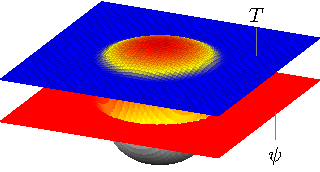
\includegraphics{figures/LinearResponse_bump}
  \caption{Illustration of Luttinger's solution to heat transport. To include a temperature fluctuation $T$, couple the system to some (fictions) gravitational potential $\psi$ giving the same current response as the temperature fluctuation.}
  \label{fig:luttinger-idea}
\end{figure}

A temperature gradient, together with external electric potential $\phi$ and chemical potential $\mu$, gives a response in the electrical current $\vec{j}$ and energy current $\vec{j}_E$~\cite{mahanManyparticlePhysics2000} 
\begin{align}
\label{eq:17}
  j_{\alpha} &= -M_{\alpha\beta}^{(11)} \left[
  \frac{e}{T} \nabla_{\beta} \phi + \nabla_{\beta} \left( \frac{\mu}{T} \right)
  \right]
  + M_{\alpha\beta}^{(12)} \nabla_{\beta} \left( \frac{1}{T} \right),\\
  J_{E,\alpha} &= -M_{\alpha\beta}^{(21)} \left[
\frac{e}{T}\nabla_{\beta}\phi + \nabla_{\beta} \left( \frac{\mu}{T} \right)
  \right] 
  + M_{\alpha\beta}^{(22)} \nabla_{\beta} \left( \frac{1}{T} \right).
\end{align}
Or, more compactly, 
\begin{equation}
  \begin{pmatrix}
    j_{\alpha } \\ j_{E,\alpha }
  \end{pmatrix}
  =
  -M_{\alpha \beta }
  \begin{pmatrix}
    \frac{e}{T}\nabla _{\beta }\phi  + \nabla _{\beta }\left( \frac{\mu}{T} \right) \\
    \nabla _{\beta }\left( \frac{1}{T} \right)
  \end{pmatrix}.
\end{equation}
The coefficients of transportation, $M_{\alpha \beta }^{(ij)}$ is a widely used convention.
The success of Luttinger's method was that the transport coefficients $M_{\alpha \beta }^{(ij)}$ could now be calculated directly, and yielded the same results as had previously been found by less formal approaches.

By the introduction of the Hamiltonian perturbation $H_L$, the response may now be investigated in the Kubo formalism.
By the response in Eq. (\ref{eq:lin-response-1}) the electric current generated from the gravitational perturbation is
% \begin{equation}
%   \label{eq:current-from-gravity}
%   \braket{\vec{J}^i}(t, \vec{r}) =
% \int \mathrm{d}t' \mathrm{d} \vec{r'} \left\{
%   \frac{-i}{\hbar} \Theta(t-t') \Braket{\left[
% \vec{J}^i(t, \vec{r}), T^{00}(t', \vec{r'})
%     \right]}
% \right\} 
% g_{00}(t', \vec{r'}),
% \end{equation}
\begin{equation}
  \label{eq:current-from-gravity}
  \braket{\vec{J}^i}(t, \vec{r}) =
\int \mathrm{d}t' \mathrm{d} \vec{r'} \left\{
  \frac{-i}{\hbar} \Theta(t-t') \Braket{\left[
\vec{J}^i(t, \vec{r}), T^{00}(t', \vec{r'})
    \right]}
\right\} 
\psi (t', \vec{r'}),
\end{equation}
where the integration is taken over the entire spacetime.
In order to express this as a response to the thermal gradient, we wish to get the gradient of the gravitational potential.
To do this, firstly the $00$-element of the stress-energy tensor will be expressed in terms derivatives of $T^{j0}$, and then a partial integration will swap the derivative between the stress-energy tensor and gravitational potential.
Note first that in the flat system the conservation law of the  energy and momentum is simply
\begin{equation}
  \partial _0 T^{00}(t, \vec{r}) + v_F \partial _i T^{i0} (t, \vec{r}) = 0,
\end{equation}
where $v_F$ is the Fermi velocity.
By the fundamental theorem of calculus this obviously gives for the zero-zero component of the stress-energy tensor
\begin{equation}
  \label{eq:18}
  T^{00}(t, \vec{r}) = - \int\limits_{-\infty }^t \mathrm{d}t'
  v_F \partial _i T^{i 0}(t', \vec{r}).
\end{equation}
Introduce Eq. (\ref{eq:18}) in the response relation (\ref{eq:current-from-gravity}), and use integration by parts
\begin{equation}
  \int u v' = uv - \int u' v,
\end{equation}
giving
\begin{equation}\label{eq:current-luttinger-gravity-final}
  \braket{\vec{J}^i}(t, \vec{r}) =
  \int \mathrm{d}t' \mathrm{d} \vec{r'}
  \int\limits_{-\infty }^{t'} \mathrm{d}t''
  \left\{
    \frac{-i v_{F}}{\hbar} \Theta(t-t') \Braket{\left[
        \vec{J}^i(t, \vec{r}), T^{j0}(t'', \vec{r'})
      \right]}
  \right\} 
  \partial'_j \psi (t', \vec{r'}).
\end{equation}
By Luttinger's relation
\begin{equation}\label{eq:current-luttinger-final}
  \braket{\vec{J}^i}(t, \vec{r}) =
  \int \mathrm{d}t' \mathrm{d} \vec{r'}
  \int\limits_{-\infty }^{t'} \mathrm{d}t''
  \left\{
    \frac{i v_{F}}{\hbar} \Theta(t-t') \Braket{\left[
        \vec{J}^i(t, \vec{r}), T^{j0}(t'', \vec{r'})
      \right]}
  \right\} 
  \frac{
    \partial'_j T (t', \vec{r'})}{
    T(t', \vec{r'})
  },
\end{equation}
where care must be taken to distinguish the stress-energy tensor $T^{j0}$ and the temperature $T$, differentiated by the indices, or lack thereof.
\todo{Check the sign here. Depending on how we understand Luttinger's method, it should be positive or negative.}


% \todo{The following section might  be moved. If we want it, need to unify. See park}
% In the interest of expressing  the gravitational potential in terms of the metric tensor, recall that in the Newtonian limit of general relativity, corresponding to $v /c \to 0$, the metric reduces to~\cite{kachelriessQuantumFieldsHubble2018}
% \begin{equation}
%   \mathrm{d}s^2 = \left( 1 + 2\psi  \right) \mathrm{d}t^2 - \left( 1 - 2 \psi  \right) \left( \mathrm{d}x^2 + \mathrm{d}y^2 + \mathrm{d}z^2 \right),
% \end{equation}
% with $\psi $ being the well-known Newtonian gravitational potential.
% Thus, we see that, remembering the definition of the line element $ds = g_{\mu \nu } \mathrm{d}x^{\mu } \mathrm{d}x^{\nu }$,
% \begin{equation}
%   g_{00} = 1 + 2\psi.
% \end{equation}
% One may therefore equivalently to Eq. (\ref{eq:current-from-gravity}) consider the response to variations of the metric component $g_{00}$ giving a term in the Hamiltonian
% \begin{equation}
%   H_L' = \int \mathrm{d}\vec{r}  \frac{g_{00}}{2} T^{00}
% \end{equation}
% with response 
% \begin{equation}
%   \braket{\vec{J}^i}(t, \vec{r}) =
% \int \mathrm{d}t' \mathrm{d} \vec{r'} \left\{
%   \frac{-i}{\hbar} \Theta(t-t') \Braket{\left[
% \vec{J}^i(t, \vec{r}), T^{00}(t', \vec{r'})
%     \right]}
% \right\} 
% \frac{\psi (t', \vec{r'})}{2},
% \end{equation}
% where the two response functions are equal.

% \todo{There is something wrong here. See park et al etc. What happens in the determinant?}
